\chapter{Results}\label{chapter:results}

This chapter measures whether a micro-frontend architecture with GraphQL and a shared caching layer can provide a performance improvement over a separated cache. In total, the micro-frontend architecture implements four \acp{SPA} and nine widgets. The major part of the implementation was done using Angular, but one single widget was implemented in React. This was done to showcase whether the shared caching layer could be used with every technology. Furthermore, a \ac{BFF} service was developed in GraphQL that is tailored to the needs of the micro-frontends. The \ac{BFF} service is used to aggregate the data from the microservices and to provide it to the micro-frontends. An overview of the prototypical architectures communicates with the GraphQL \ac{API} is shown in listing \ref{fig:results:micro-frontend-prototype}.

\ifshowImages
\begin{figure}[H]
  \centering
  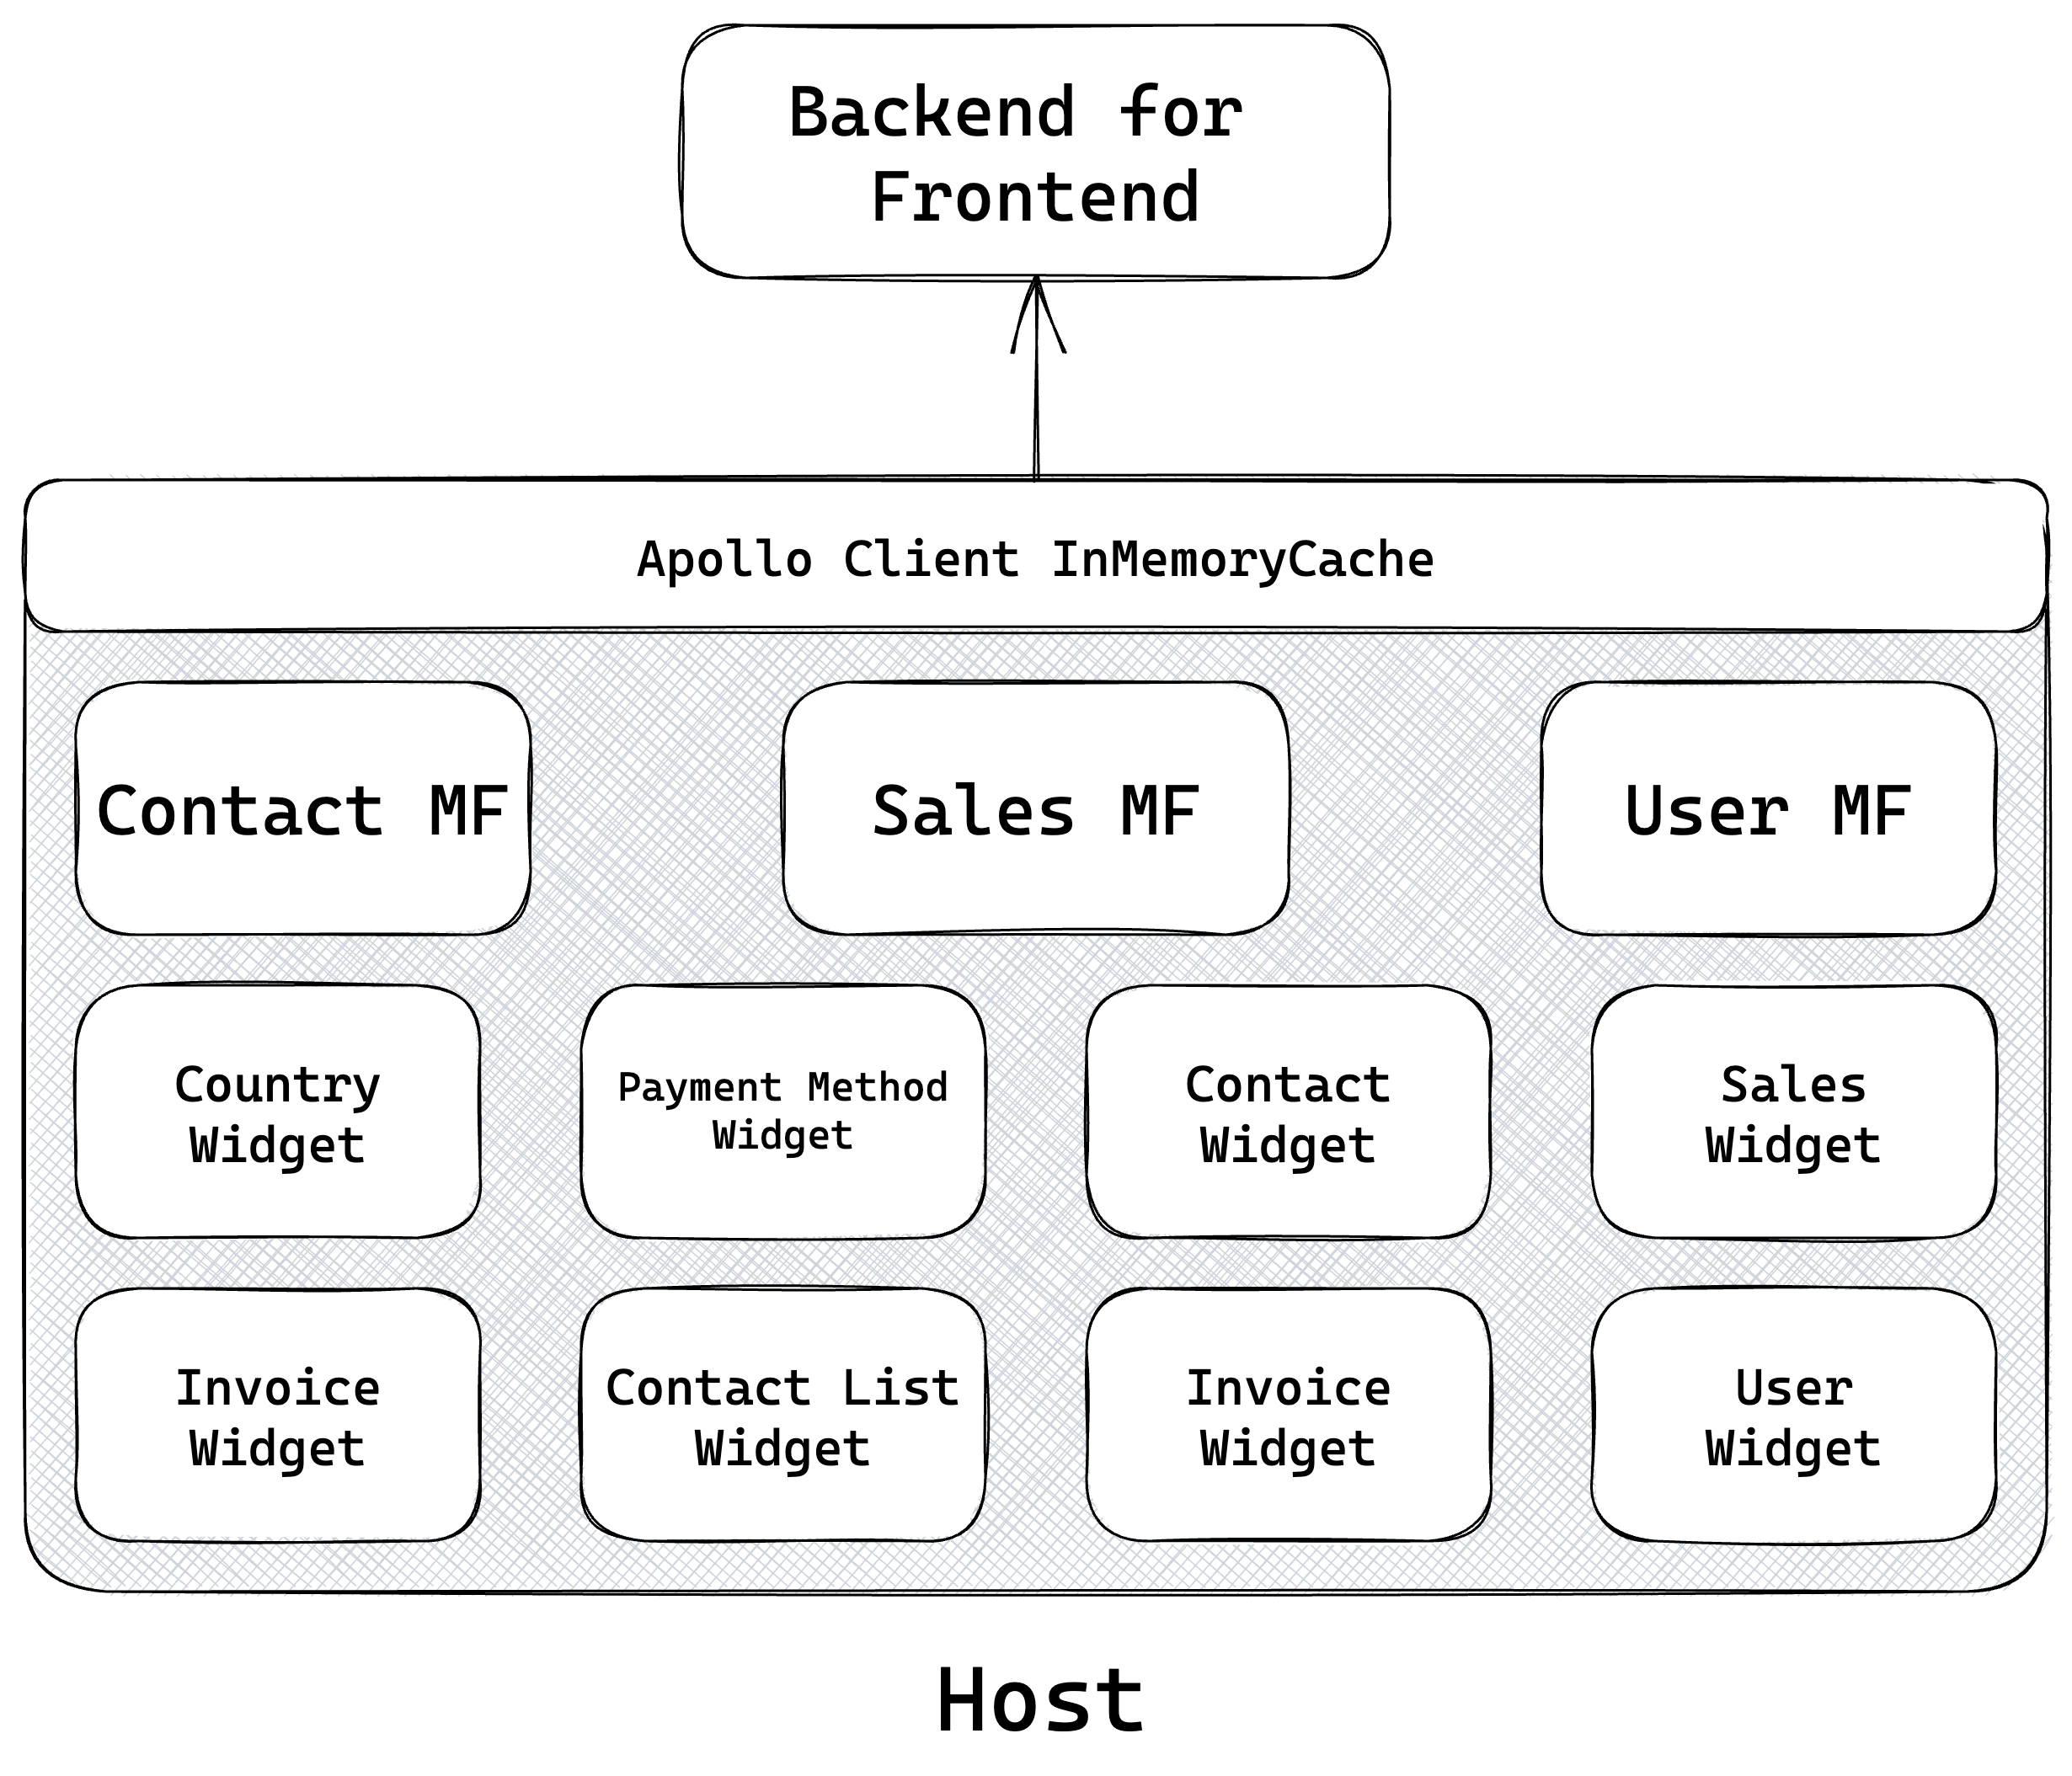
\includegraphics[width=0.8\linewidth]{images/results/micro-frontend-prototype.png}
  \caption{Architecture of the micro-frontend prototype.}\label{fig:results:micro-frontend-prototype}
\end{figure}
\fi

\section{Performance measurement}\label{section:results:performance-measurement}

This section explains how the micro-frontend architecture was evaluated in terms of the hypothesis. Three distinct approaches were identified to measure the performance of the shared GraphQL caching layer. The architecture allows switching easily between these three approaches.

\begin{enumerate}
  \item \textbf{Separate Cache and no reduced queries}: All remote modules use a separate cache and no queries are reduced with the help of the cache.
  \item \textbf{Shared Cache and no reduced queries}: The remote modules share the same cache instance and no queries are reduced with the help of the cache.
  \item \textbf{Shared Cache and reduced queries}: ALL remote modules share the same instance of the cache and queries are reduced by utilizing the cache.
\end{enumerate}

\noindent To measure and compare the performance of these three approaches, two exemplary paths through the application were planned. These paths were intended to show how many network requests were made to the GraphQL \ac{API} and how much network traffic was generated in the process. To make the measurement as close as possible to a real application, a large amount of mock data was generated for the GraphQL \ac{API}. With this large amount of data, it is easier to measure the differences in response size. Smaller datasets only make a big difference, if the application is used for longer periods. The next section details the results of the first path through the application.

\subsection{Evaluation}\label{subsection:results:performance-measurement:evaluation}

This section describes how the shared caching layer and the reduction of queries were tested for the prototypical micro-frontend architecture. It explains the user journey through the application and shows the results for the three different approaches. The figure \ref{fig:results:evaluation-first-path} shows the steps through the micro-frontend architecture that were used to measure the possible performance improvements of the shared caching layer and the reduction of queries. The client has to perform 13 steps throughout the application, which involves almost every available GraphQL query. The dashoard yields some problems, when starting the evaluation there. All widgets are created and start to fetch their data at the same time. Therefore, it can easily happen that multiple widgets fetch the same queries from the GraphQL \ac{API} because the data is not already in the cache. This is a problem that is difficult to circumvent and leads to a lot of theoretically unnecessary network requests. The evaluation is performed with an unauthenticated user.

\ifshowImages
\begin{figure}[H]
\centering
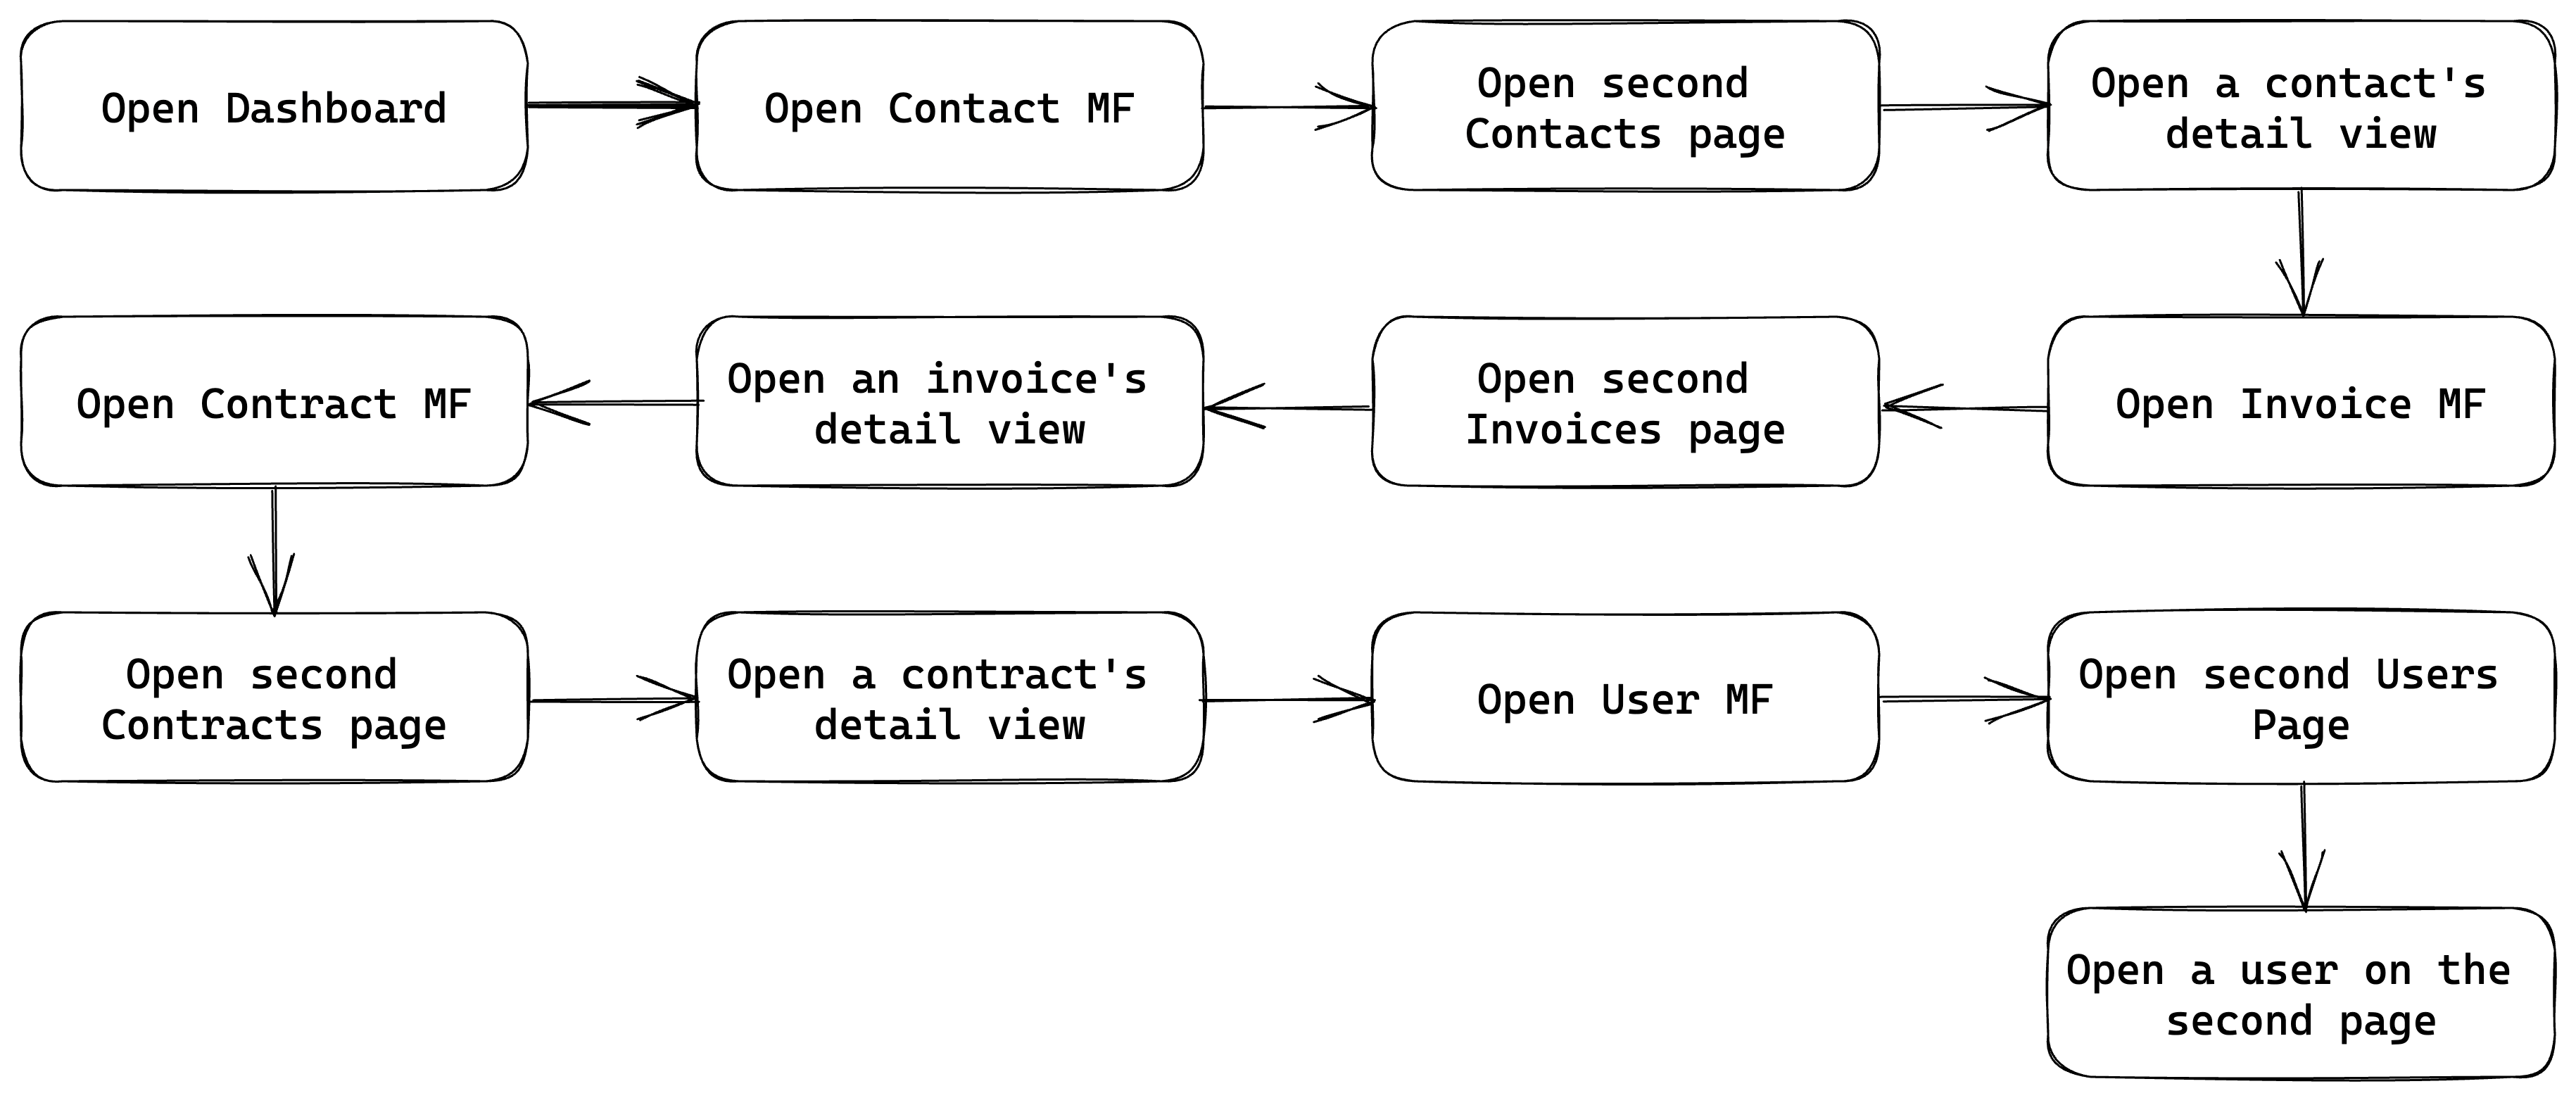
\includegraphics[width=1\linewidth]{images/results/evaluation-first-path.png}
\caption{A user journey through the application to measure the performance of the micro-frontend architecture.}\label{fig:results:evaluation-first-path}
\end{figure}
\fi

\noindent Without the use of a caching system, the GraphQL \ac{API} would have to run 59 queries to provide the data for the path through the application. How the prototypical micro-frontend architecture can be configured to use one of the three approaches is already explained in section \ref{section:applied-methods:shared-caching-layer} and section \ref{subsection:applied-methods:query-reduction:testing-query-reduction}. The following sections describe and compare the results of the approaches in more detail.

\subsubsection{Separate Cache and no reduced queries}\label{subsubsection:results:performance-measurement:separate-cache-no-reduction}

In this approach, each micro frontend has a separate instance of the GraphQL client and \texttt{InMemoryCache}. The queries are not reduced using the cache and the custom implementation. After the client completes the journey through the application, the following metrics were collected.

\begin{itemize}
  \item 47 network requests to the GraphQL \ac{API}
  \item 10.78MB transferred
\end{itemize}

\noindent The \texttt{GRAPHQL\_CLIENT\_OPTIONS\_CONFIG} and \texttt{REDUCE\_QUERY\_OPTIONS} injection tokens have to be configured the following way A more detailed description of the configuration options can be found in section \ref{section:applied-methods:shared-caching-layer} and in section \ref{subsection:applied-methods:query-reduction:testing-query-reduction}:

\begin{itemize}
  \item \texttt{shareCache: false}
  \item \texttt{reduceQueries: false}
\end{itemize}

\noindent 47 network requests have to be made to the GraphQL backend which can be seen in figure \ref{fig:results:no-shared-cache-no-reduction}. The figure shows 53 requests in total, but six requests have to be subtracted because they are needed to make the prototypical architecture work. They load the micro-frontends from their remote locations and fetch their settings. These requests are only needed for the functionality of the micro-service architecture.

\ifshowImages
\begin{figure}[H]
\centering
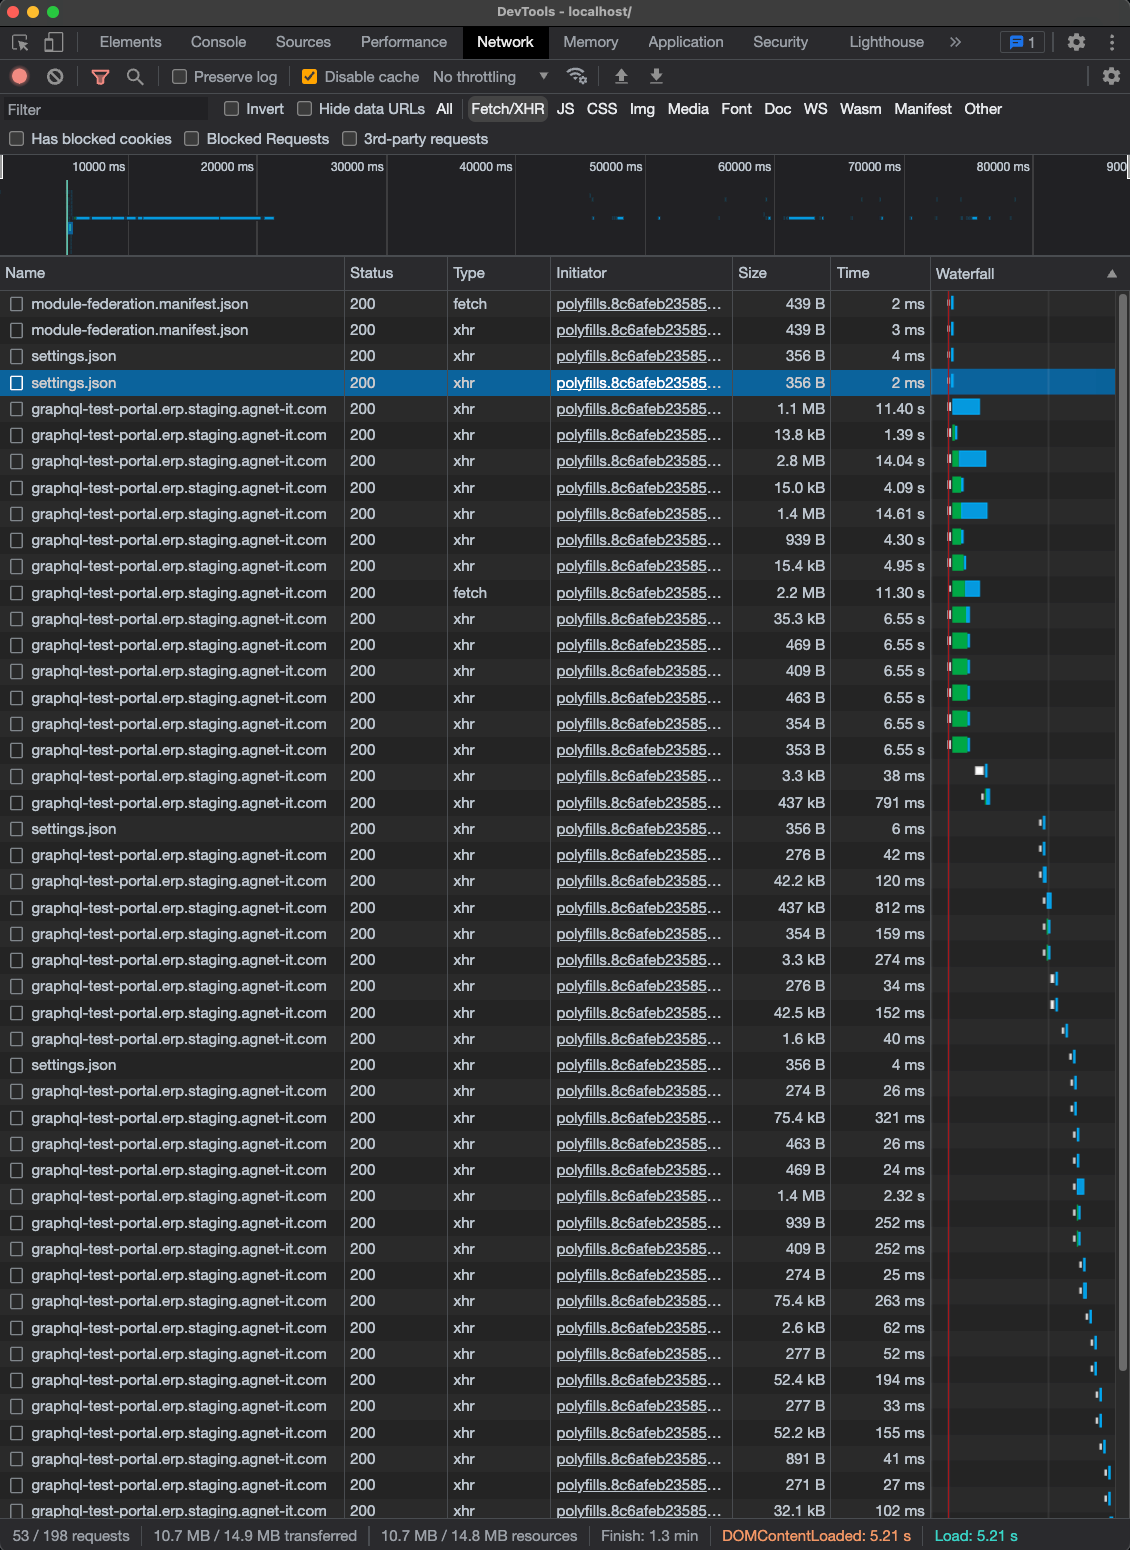
\includegraphics[width=0.6\linewidth]{images/results/1-attempt/no-shared-cache-no-reduction.png}
\caption{All requests made during the measurement of the first approach.}\label{fig:results:no-shared-cache-no-reduction}
\end{figure}
\fi

\noindent The total size of the requests was 17.46 KB and the size of the responses was 10.78 MB. The 47 queries retrieve a total of 81510 records from the GraphQL backend.

\subsubsection{Shared Cache and no reduced queries}\label{subsubsection:results:performance-measurement:shared-cache-no-reduction}

In this approach, an instance of the cache is shared by all micro-frontends, but the GraphQL queries are not reduced with data already present in the \texttt{InMemoryCache}. After the client completes the journey through the application, the following metrics were collected:

\begin{itemize}
  \item 36 network requests to the GraphQL \ac{API}
  \item 8.5 MB transferred
\end{itemize}

\noindent The \texttt{GRAPHQL\_CLIENT\_OPTIONS\_CONFIG} and \texttt{REDUCE\_QUERY\_OPTIONS} injection tokens have to be configured the following way:

\begin{itemize}
  \item \texttt{shareCache: true}
  \item \texttt{reduceQueries: false}
\end{itemize}

\noindent 36 requests have to be made to the GraphQL backend which can be seen in figure \ref{fig:results:no-shared-cache-no-reduction}. Six requests have to be deducted (\texttt{settings.json}, \texttt{module-federation.manifest.json}, \dots) like in the previous section.

\ifshowImages
\begin{figure}[H]
\centering
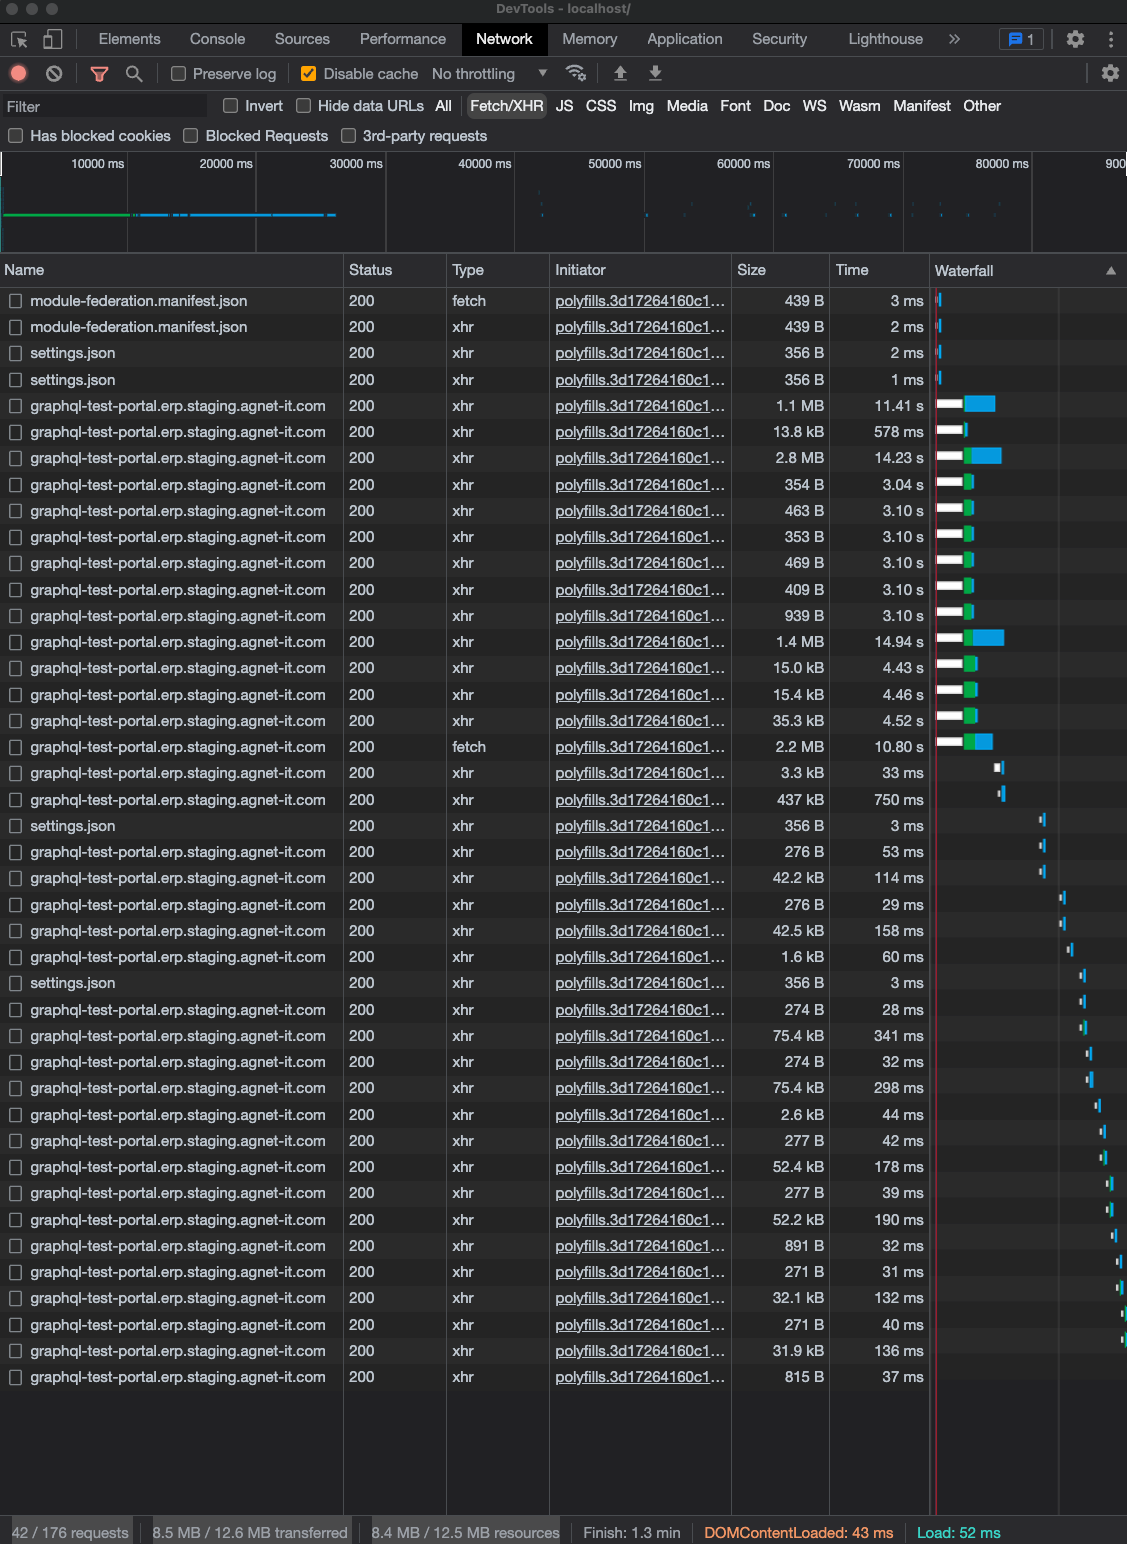
\includegraphics[width=0.6\linewidth]{images/results/1-attempt/shared-not-reduced-cache.png}
\caption{All requests made during the measurement of the second approach.}\label{fig:results:shared-cache-no-reduction}
\end{figure}
\fi

\noindent The total size of the queries was 15.176 KB and the size of the responses was 8.5 MB. The 36 queries retrieve a total of 51319 records from the GraphQL backend.

\subsubsection{Shared cache, query reduction}\label{subsubsection:results:performance-measurement:separate-cache-reduction}

With this approach, the same instance of the cache is shared between all of the micro-frontends in the architecture, and the queries are reduced with already existing data inside the cache. After the client completes the journey through the application, the following metrics were collected.

\begin{itemize}
  \item 36 network requests to the GraphQL \ac{API}
  \item 8.4 MB transferred
\end{itemize}

\noindent The \texttt{GRAPHQL\_CLIENT\_OPTIONS\_CONFIG} and \texttt{REDUCE\_QUERY\_OPTIONS} injection tokens have to be configured the following way:

\begin{itemize}
  \item \texttt{shareCache: true}
  \item \texttt{reduceQueries: true}
\end{itemize}

\noindent 36 requests have to be made to the GraphQL backend which can be seen in figure \ref{fig:results:no-shared-cache-no-reduction}. Six requests have to be deducted (\texttt{settings.json}, \texttt{module-federation.manifest.json}, \dots) like in the previous sections.

\ifshowImages
\begin{figure}[H]
\centering
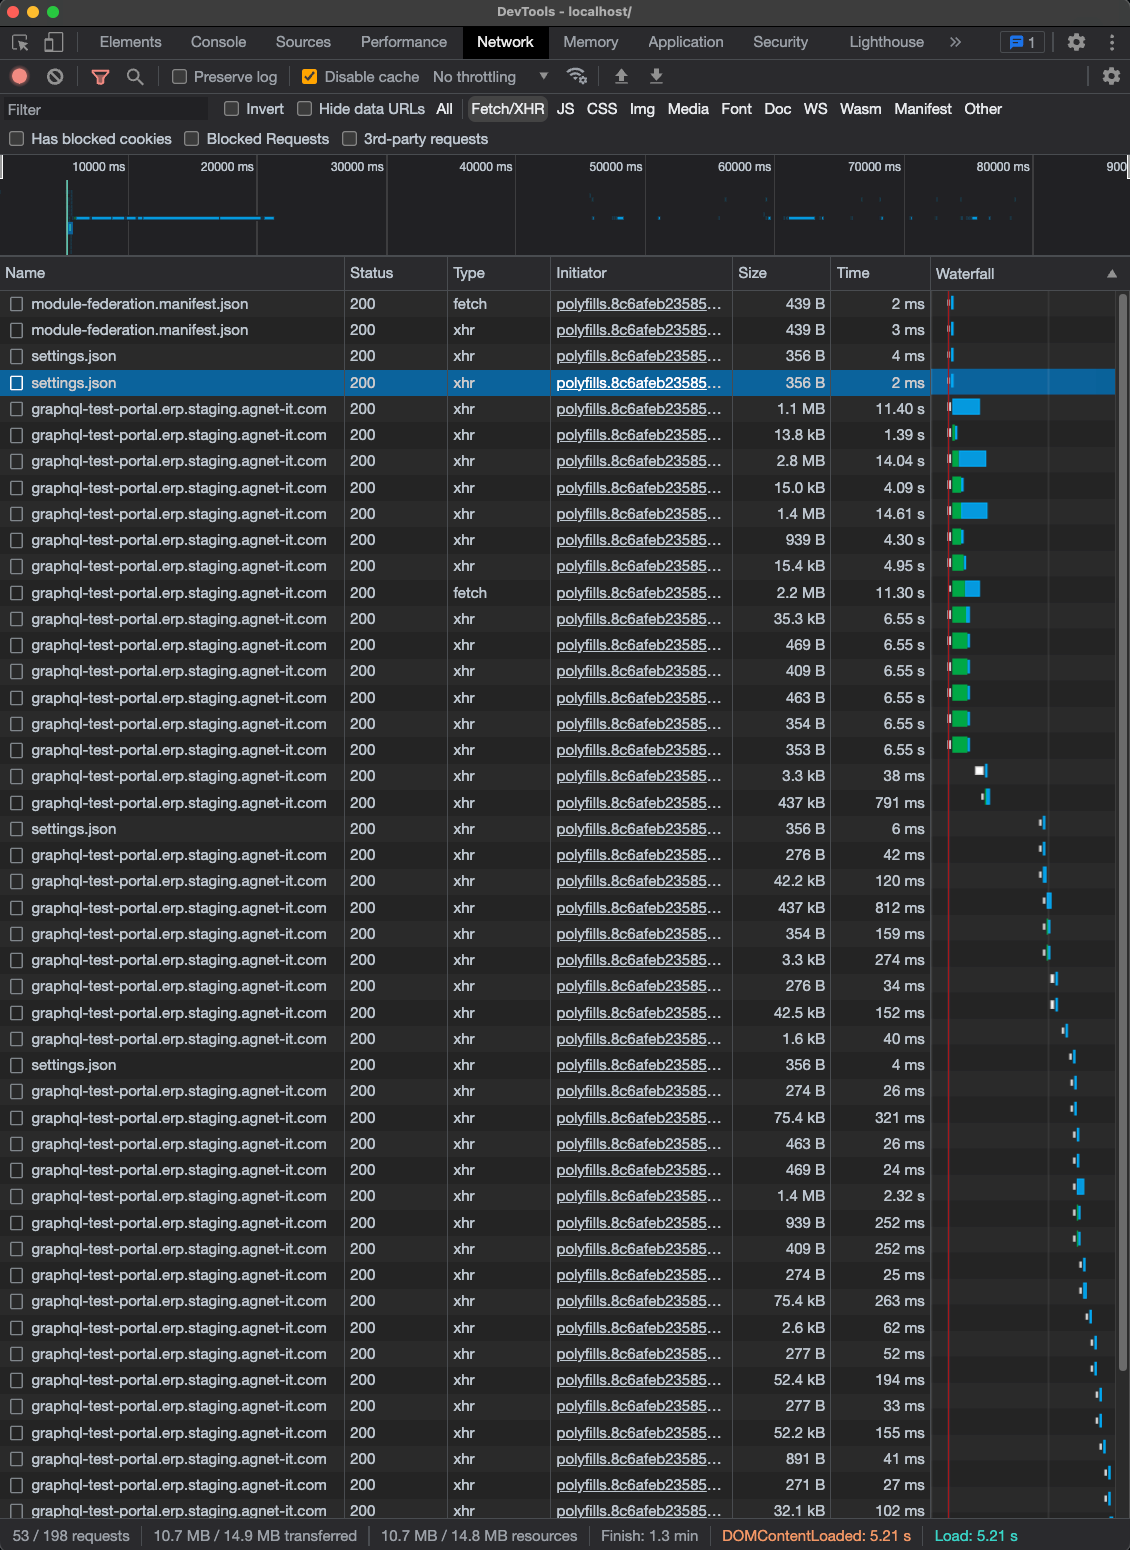
\includegraphics[width=0.6\linewidth]{images/results/1-attempt/no-shared-cache-no-reduction.png}
\caption{All requests made during the measurement of the third approach.}\label{fig:results:shared-cache-reduction}
\end{figure}
\fi

\noindent The total size of the queries was 13.533 KB and the size of the responses was 8.37 MB. The 36 queries retrieve a total of 51319 records from the GraphQL backend.

\section{Comparing the results of the first user journey}\label{section:results:comparison-first-journey}

This section takes the measurements from the previous section \ref{subsection:results:performance-measurement:evaluation} and compares the different approaches in terms of request sizes and response sizes, the number of requests, and the total records fetched.

\subsection{Comparing the first- and second-approach}\label{subsection:results:comparison-first-second-approach}

When comparing the first- with the second approach there is a significant difference in the number of network requests made to the GraphQL \ac{API} and the size of the requests and responses, as seen in table \ref{table:results:size-comparison-first-path-no-cache-no-reduction-cache-no-reduction}. The shared cache approach requires eleven fewer network requests than the separate cache approach. Since the queries are not reduced for this comparison, the additional network queries account for the overall difference in request- and response size. The 11 additional requests from the first approach send an additional 2.29 KB to the backend and return about an additional 2.34 MB from the backend. Therefore, 22\% of the total response size can be saved by using only one shared cache for all micro-frontends. Another interesting observation is that the shared cache approach retrieves 30191 fewer records than the naive approach, which is about 37\% of the total records returned.

\ifshowTables
\begin{table}[H]
  \begin{tabular}{|l|l|l|l|l|}
  \hline
    & \textbf{Request Size (B)} & \textbf{Response Size (B)} & \textbf{Requests} & \textbf{Records} \\
    \hline
    \textbf{No Reduction, Separate Cache} & 17462 & 10780656 & 47 & 81510 \\
    \hline
    \textbf{No Reduction, Shared Cache} & 15176 & 8437211 & 36 & 51319 \\
    \hline
    \hline
    \textbf{Diff} & \textbf{2286} & \textbf{2343445} & \textbf{11} & \textbf{30191} \\
    \hline
    \textbf{Reduction (\%)} & \textbf{13\%} & \textbf{22\%} & \textbf{23\%} & \textbf{37\%} \\
    \hline
  \end{tabular}
  \caption{First Journey: Comparing the requests and responses of the first- and second-approach.}\label{table:results:size-comparison-first-path-no-cache-no-reduction-cache-no-reduction}
\end{table}
\fi

\noindent The following enumeration shows which and how often GraphQL queries were dropped when using a shared caching layer between the micro front-ends compared to a separate cache:

\begin{itemize}
  \item allCountries: 2
  \item allSalutations: 2
  \item allTitles: 2
  \item allArticleUnits: 1
  \item allCurrencies: 1
  \item allVats: 1
  \item allSalesCountries: 1
  \item allInvoiceTypes: 1
\end{itemize}

\noindent The data of the requests that were omitted is usually used for filling selection controls inside detail views and has to be fetched over and over again in every micro-frontend. The first three queries are used for widgets on the dashboard, the contact application, and the user application. The last five queries are used for widgets on the dashboard and the sales application.

\subsection{Comparing the first- and third-approach}\label{subsection:results:comparison-first-third-approach}

Like in the previous comparison, there is the same difference in the number of network requests made to the GraphQL \ac{API}. The size of the responses and the requests have a massive difference, just like before. The results are shown in table \ref{table:results:size-comparison-first-path-no-cache-no-reduction-cache-reduction}. Just like before, there is a difference of 11 GraphQL queries that are sent to the GraphQL \ac{API}. However, due to the reduction in queries, the difference in the size of the queries and responses is greater than in section \ref{subsection:results:comparison-first-second-approach}. All queries of the first approach send 3.92 KB more and return about 2.41 MB more from the GraphQL \ac{API} compared to the third approach. A shared cache and query reduction can save about 22\% response sizes. As before, 37\% fewer records need to be fetched from the backend.

\ifshowTables
\begin{table}[H]
  \begin{tabular}{|l|l|l|l|l|}
  \hline
  & \textbf{Request Size (B)} & \textbf{Response Size (B)} & \textbf{Requests} & \textbf{Records}  \\
  \hline
  \textbf{No Reduction, Separate Cache} & 17462 & 10780656 & 47 & 81510 \\
  \hline
  \textbf{Reduction, Shared Cache} & 13533 & 8374763 & 36 & 51319 \\
  \hline
  \hline
  \textbf{Diff} & \textbf{3929} & \textbf{2405893} & \textbf{11} & \textbf{30191} \\
  \hline
  \textbf{Reduction (\%)} & \textbf{23\%} & \textbf{22\%} & \textbf{23\%} & \textbf{37\%} \\
  \hline
  \end{tabular}
  \caption{First Journey: Comparing the requests and responses of the first- and third-approach.}\label{table:results:size-comparison-first-path-no-cache-no-reduction-cache-reduction}
\end{table}
\fi

\subsection{Comparing the second- and third-approach}\label{subsection:results:comparison-second-third-approach}

Between the first- and the second approach, there is almost no difference in terms of request- and response size compared to the comparisons from section \ref{subsection:results:comparison-first-second-approach} and \ref{subsection:results:comparison-first-third-approach}, as seen in table \ref{table:results:size-comparison-first-path-no-cache-no-reduction-cache-reduction}. Both approaches have the same number of queries sent to the GraphQL \ac{API} since the cache is shared by all micro-frontends. Reducing queries does not lead to fewer network requests. The difference in request and response size between the two approaches comes solely from the use of query reduction. By using the third approach, the difference in request size is about 1.64 KB (11\%), which is not significant. The difference between the response sizes (62.45 KB) is almost zero in relation to the amount of data that was returned.

\ifshowTables
\begin{table}[H]
  \begin{tabular}{|l|l|l|l|l|}
  \hline
  & \textbf{Request Size (B)} & \textbf{Response Size (B)} & \textbf{Requests} & \textbf{Records} \\
  \hline
  \textbf{No Reduction, Shared Cache} & 15176 &  8437211 & 36 & 51319 \\
  \hline
  \textbf{Reduction, Shared Cache} &  13533 &  8374763 & 36 & 51319 \\
  \hline
  \hline
  \textbf{Diff} & \textbf{1643} & \textbf{62448} & \textbf{0} & \textbf{0} \\
  \hline
  \textbf{Reduction (\%)} & \textbf{11\%} & \textbf{0\%} & \textbf{-} & \textbf{-} \\
  \hline
  \end{tabular}
  \caption{First Journey: Comparing the requests and responses of the second- and third-approach.}\label{table:results:size-comparison-first-path-cache-no-reduction-cache-reduction}
\end{table}
\fi

\section{Compare the results of the second user journey}\label{section:results:comparison-second-journey}

This section compares the results for a second user journey through the prototype between the three approaches explained in Section \ref{section:results:performance-measurement}. The client's journey through the application is shown in Figure \ref{fig:results:evaluation-second-path}. The client has to perform 17 steps throughout the prototype, which involves running every available GraphQL query. In contrast to the first journey from Section \ref{section:results:comparison-first-journey}, the client uses an authenticated user to perform the test. The GraphQL \ac{API} query to retrieve the authenticated user is performed by every micro-frontend individually.

\ifshowImages
\begin{figure}[H]
  \centering
  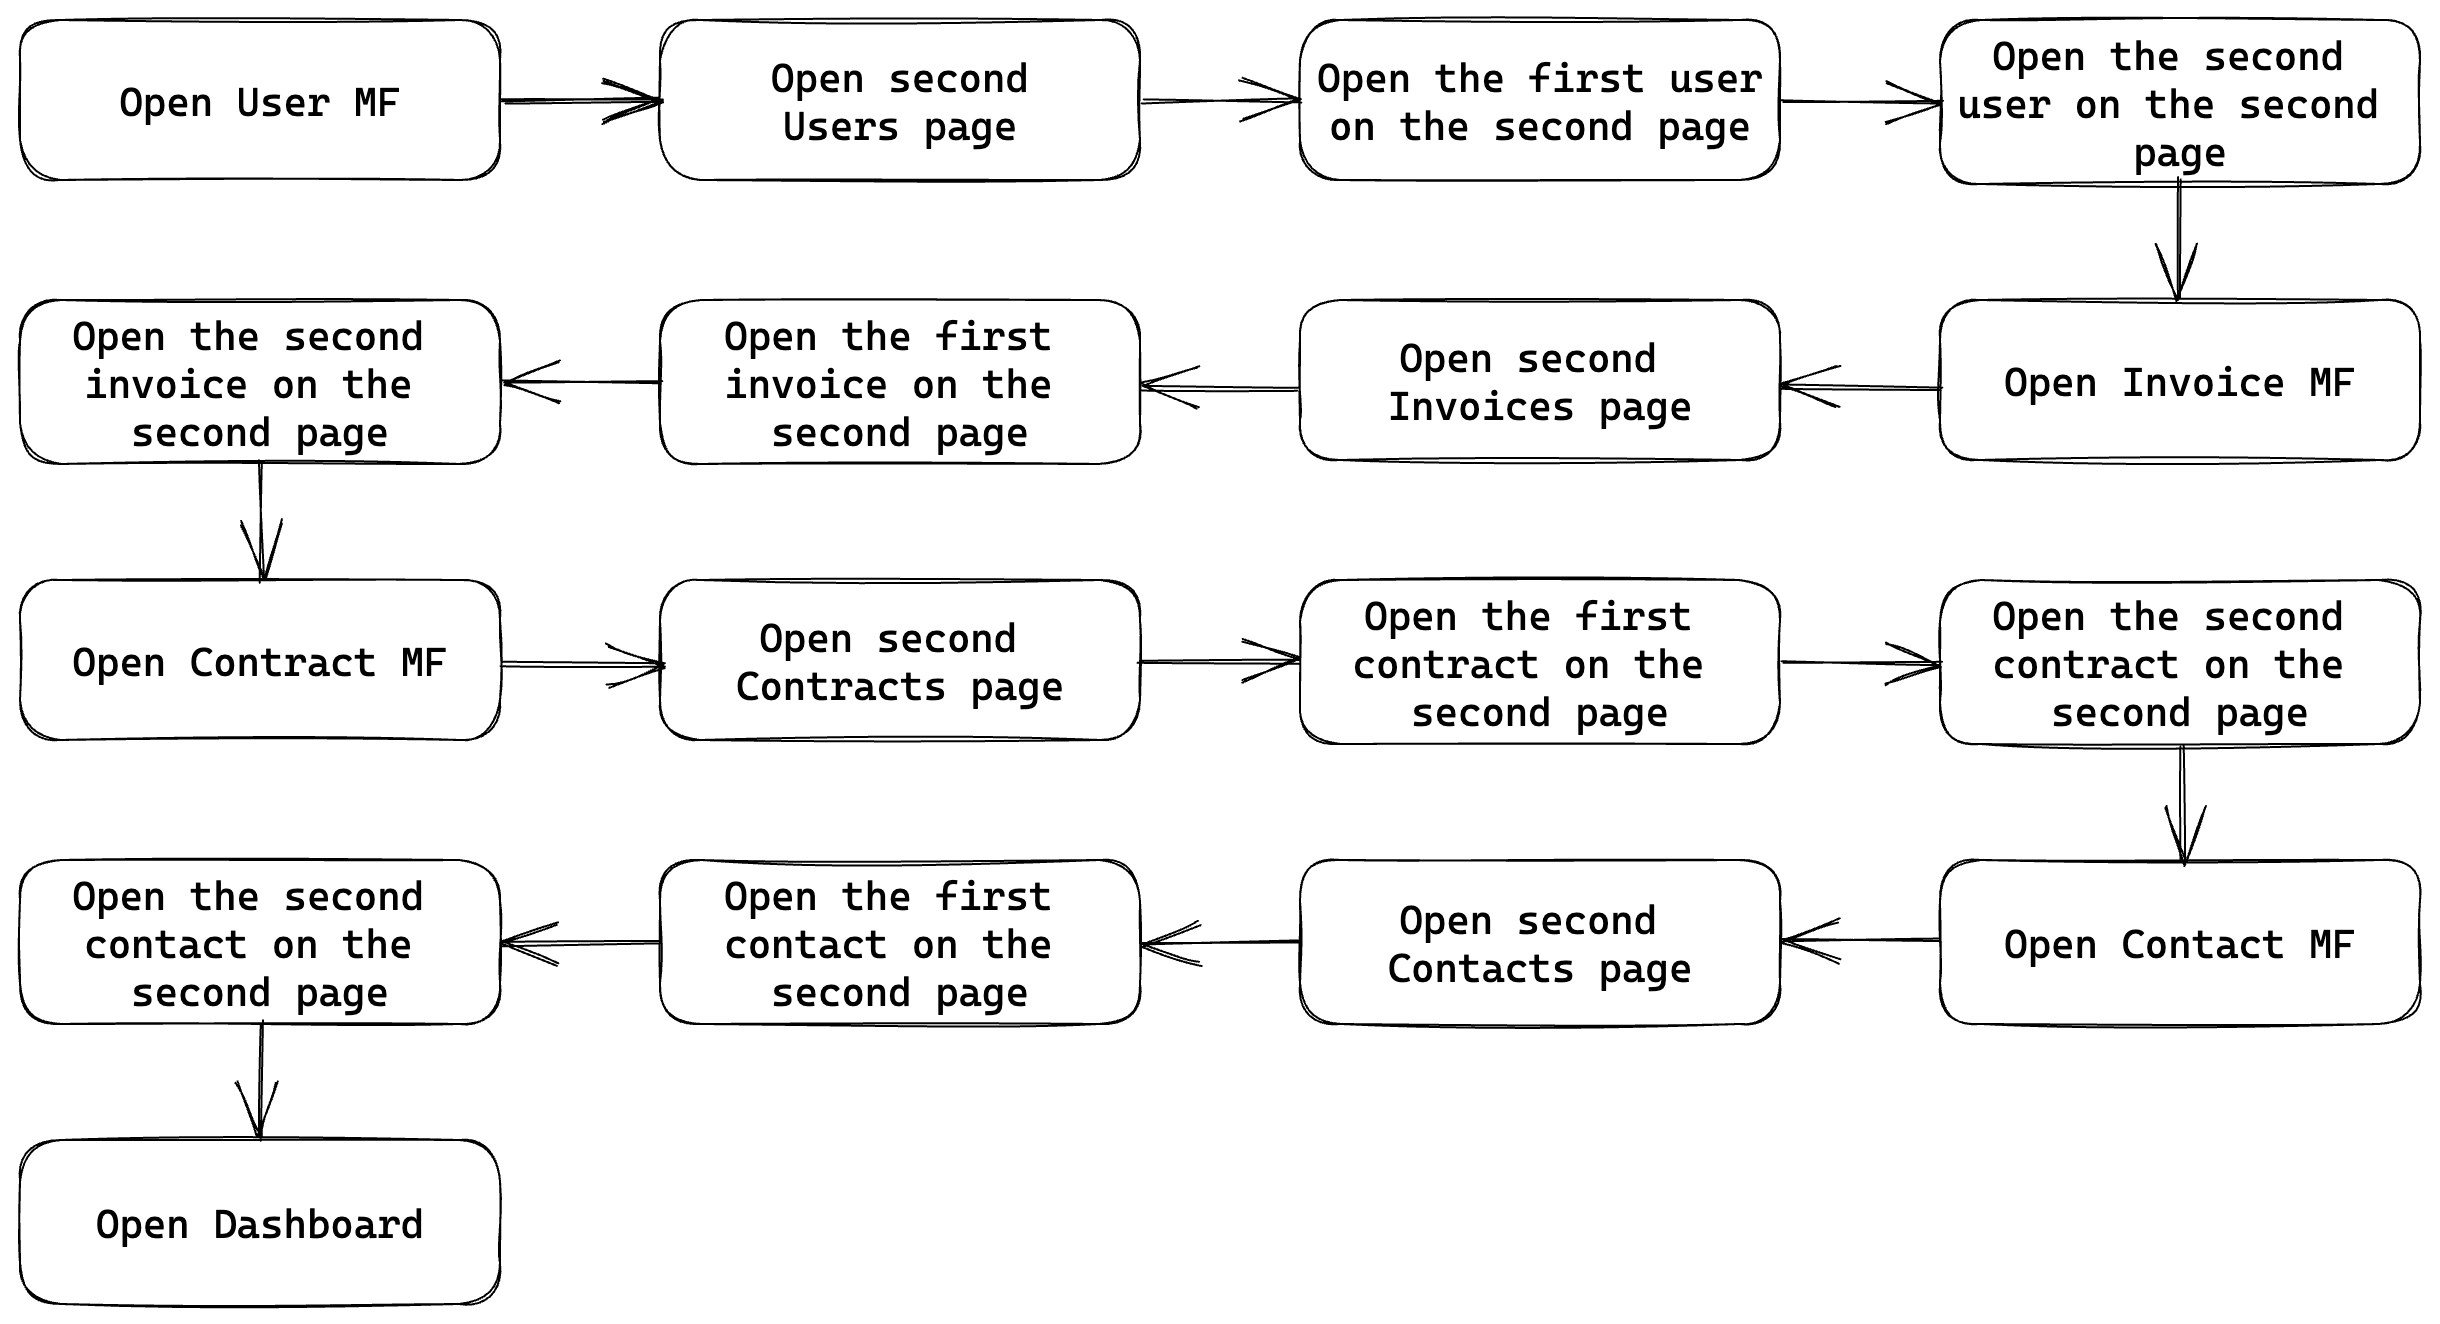
\includegraphics[width=1\linewidth]{images/results/evaluation-second-path.png}
  \caption{The second user journey through the application to measure the performance of the micro-frontend architecture.}\label{fig:results:evaluation-second-path}
\end{figure}
\fi

\noindent The following sections compare the three distinct approaches regarding request size, response size, number of requests, and the total number of records fetched, just as in the previous Section \ref{section:results:comparison-first-journey}.

\subsection{Compare the first- and second-approach}\label{subsection:results:comparison-second-path-first-second-approach}

Comparing the first approach with the second, there is a difference of 25 network requests to the GraphQL \ac{API} and the size of the requests and responses, as seen in Table \ref{table:results:size-comparison-second-path-cache-no-reduction-cache-reduction}. The second approach requires 25 fewer network requests than the first approach. Since the queries are not altered for this comparison, the additional network requests are responsible for the overall difference in request- and response size. The difference in request size is 26\%, which is about 6.07 KB, which is insignificant. Using a shared cache layer can save about 22\% of the total response size. Another interesting observation is that the shared cache approach retrieves 30401 fewer records than the naive approach, which is about 37\% of the total records returned.

\ifshowTables
\begin{table}[H]
  \begin{tabular}{|l|l|l|l|l|}
  \hline
  & \textbf{Req. size (B)} & \textbf{Resp. size (B)} & \textbf{Requests} & \textbf{Records} \\
  \hline
  \textbf{No Reduction, Separate Cache} & 22955 & 10713304 & 62 & 81325 \\
  \hline
  \textbf{No Reduction, Shared Cache} & 16884 & 8364416 & 37 & 50924 \\
  \hline
  \hline
  \textbf{Diff (B)} & \textbf{6071} & \textbf{2348888} & \textbf{25} & \textbf{30401} \\
  \hline
  \textbf{Reduction (\%)} & \textbf{26\%} & \textbf{22\%} & \textbf{40\%} & \textbf{37\%} \\
  \hline
  \end{tabular}
  \caption{Second Journey: Compare the requests and responses of the second- and third-approach.}\label{table:results:size-comparison-second-path-cache-no-reduction-cache-reduction}
\end{table}
\fi

\subsection{Compare the first- and third-approach}\label{subsection:results:comparison-second-path-second-third-approach}

As in the previous comparison, there are again 25 requests less made to the GraphQL \ac{API}. The size of the responses and the requests are similar to the previous section. The results are shown in Table \ref{table:results:size-comparison-second-path-no-cache-no-reduction-cache-reduction}. However, due to the reduction in queries, the difference in the size of queries and responses is more pronounced than in Section \ref{subsection:results:comparison-second-path-first-second-approach}. The difference in request size is 36\%, which accounts for 8.24 KB, which is insignificant. A shared caching layer and query reduction can save about 22\% of response size; as before, 37\% fewer records need to be fetched from the GraphQL \ac{API}.

\ifshowTables
\begin{table}[H]
  \begin{tabular}{|l|l|l|l|l|}
  \hline
  & \textbf{Req. size (B)} & \textbf{Resp. size (B)} & \textbf{Requests} & \textbf{Records} \\
  \hline
  \textbf{No Reduction, Separate Cache} & 22955 & 10713304 & 62 & 81325 \\
  \hline
  \textbf{Reduction, Shared Cache} & 14718 & 8361306 & 37 & 50924 \\
  \hline
  \hline
  \textbf{Diff (B)} & \textbf{8237} & \textbf{2351998} & \textbf{25} & \textbf{30401} \\
  \hline
  \textbf{Reduction (\%)} & \textbf{36\%} & \textbf{22\%} & \textbf{40\%} & \textbf{37\%} \\
  \hline
  \end{tabular}
  \caption{Second Journey: Compare the requests and responses of the first- and third-approach.}\label{table:results:size-comparison-second-path-no-cache-no-reduction-cache-reduction}
\end{table}
\fi

\subsection{Compare the second- and third-approach}\label{subsection:results:comparison-second-path-first-third-approach}

Between the second and third approaches, there is almost no difference regarding request size and response size. The results are displayed in Table \ref{table:results:size-comparison-second-path-no-cache-no-reduction-cache-no-reduction}. Both approaches have the same number of queries sent to the GraphQL \ac{API} and receive the same amount of records since all micro-frontends share the same cache instance. The difference in request and response size comes solely from using the query reduction mechanism. The difference in request size is 13\%, but they account for just 2.17 KB, which is insignificant. The difference between the response sizes (3.11 KB) is almost zero, like in the first user journey.

\ifshowTables
\begin{table}[H]
  \begin{tabular}{|l|l|l|l|l|}
  \hline
  & \textbf{Req. size (B)} & \textbf{Resp. size (B)} & \textbf{Requests} & \textbf{Records} \\
  \hline
  \textbf{No Reduction, Shared Cache} & 16884 & 8364416 & 37 & 50924 \\
  \hline
  \textbf{Reduction, Shared Cache} & 14718 & 8361306 & 37 & 50924 \\
  \hline
  \hline
  \textbf{Diff (B)} & \textbf{2166} & \textbf{3110} & \textbf{0} & \textbf{0} \\
  \hline
  \textbf{Reduction (\%)} & \textbf{13\%} & \textbf{0\%} & \textbf{-} & \textbf{-} \\
  \hline
  \end{tabular}
  \caption{Second Journey: Compare the requests and responses of the first- and second-approach.}\label{table:results:size-comparison-second-path-no-cache-no-reduction-cache-no-reduction}
\end{table}
\fi

\section{Compare original and reduced queries}

This section examines the differences in network request size and network response size between the reduced GraphQL queries and the unmodified original queries. The size difference between the original and reduced queries is calculated in percentages and bytes. Table \ref{table:code:comparison-user-reduction} shows the difference in network size for the user-detail query between the original and the reduced queries. The query fetches a user by its unique id. The network data was collected by fetching 10 different users from the GraphQL \ac{API} and looking at the request and response size. The requested fields of the user-detail query and which fields are removed fields with query reduction are explained in more detail in Section \ref{subsection:background:graphql:example-reduction}. The original query contains 16 fields, and 8 fields are removed from the query using the query reduction functionality. By removing 8 fields from the original GraphQL query, the size of the request to the GraphQL \ac{API} was reduced by about 30\% or 161 bytes. The difference in query sizes is always the same because the same 8 fields are removed from each user-detail query. When fetching 10 different users, a total of 1.61 KB of request size can be saved. The response size was reduced by 42\% on average. About 2.55 KB response size is saved when 10 different users are fetched from the GraphQL \ac{API} using query reduction. The response size difference varies slightly from user to user, because the content of the fields is different. The difference from the smallest to the largest user is only about 2\%.

\ifshowTables
\begin{table}[!htbp]
  \begin{tabular}{|l|l|l|l|l|}
  \hline
  \textbf{Query} & \textbf{Req. diff (\%)} & \textbf{Req. size diff (B)} & \textbf{Resp. diff (\%)} & \textbf{Resp. size diff (B)} \\
  \hline
  User A & 30\% & 161 & 42\% & 257 \\
  \hline
  User B & 30\% & 161 & 42\% & 257 \\
  \hline
  User C & 30\% & 161 & 41\% & 257 \\
  \hline
  User D & 30\% & 161 & 42\% & 244 \\
  \hline
  User E & 30\% & 161 & 43\% & 251 \\
  \hline
  User F & 30\% & 161 & 42\% & 271 \\
  \hline
  User G & 30\% & 161 & 42\% & 249 \\
  \hline
  User H & 30\% & 161 & 41\% & 263 \\
  \hline
  User I & 30\% & 161 & 41\% & 248 \\
  \hline
  User J & 30\% & 161 & 41\% & 252 \\
  \hline
  \hline
  \textbf{AVG} & \textbf{30\%} & - & \textbf{42\%} & -  \\
  \hline
  \hline
  \textbf{SUM} & - & \textbf{1610 (1.61 KB)} & - & \textbf{2549 (2.55 KB)} \\
  \hline
  \multicolumn{5}{l}{16 fields requested, 8 fields Removed, 8 remaining sent to the GraphQL \ac{API}}
  \end{tabular}
  \caption{A comparison of the user-detail query in request- and response-sizes.}\label{table:code:comparison-user-reduction}
\end{table}
\fi

% \bigskip

\noindent Table \ref{table:code:comparison-contract-reduction} shows the difference in network size for the contract-detail query between the original and reduced queries. The query fetches the detail data of a contract with its unique id. The network data was collected by fetching 10 different contracts. The original query contains 17 fields, where 10 fields were removed from the query using the query reduction functionality. Therefore, only 7 of the 17 fields remain within the query, which means that 58\% of the original fields were removed. The size of the requests to the GraphQL \ac{API} can be reduced by an average of 38\% or 207 bytes. Using the application and querying 10 detail views of a contract 2.07 KB of request size can be saved. The size GraphQL \ac{API} response can be reduced by about 58\% or 3.96 KB when fetching 10 different contracts. The response size savings vary slightly from contract to contract because the content of the fields is different. The difference from the smallest to the largest contract is only about 3\%.

\ifshowTables
\begin{table}[!htbp]
  \begin{tabular}{|l|l|l|l|l|}
  \hline
  \textbf{Query} & \textbf{Req. diff (\%)}  & \textbf{Req. size diff (B)} & \textbf{Resp. diff (\%)} & \textbf{Resp. size diff (B)}  \\
  \hline
  Contract A & 38\% & 207 & 58\% & 394 \\
  \hline
  Contract B & 38\% & 207 & 58\% & 378 \\
  \hline
  Contract C & 38\% & 207 & 59\% & 403 \\
  \hline
  Contract D & 38\% & 207 & 60\% & 408 \\
  \hline
  Contract E & 38\% & 207 & 60\% & 409 \\
  \hline
  Contract F & 38\% & 207 & 57\% & 370 \\
  \hline
  Contract G & 38\% & 207 & 58\% & 393 \\
  \hline
  Contract H & 38\% & 207 & 58\% & 407 \\
  \hline
  Contract I  & 38\% & 207 & 59\% & 400 \\
  \hline
  Contract J & 38\% & 207 & 58\% & 389 \\
  \hline
  \hline
  \textbf{AVG} & \textbf{38\%} & - & \textbf{58\%} & - \\
  \hline
  \hline
  \textbf{SUM} & - & \textbf{2070 (2.07 KB)} & - & \textbf{3951 (3.95 KB)} \\
  \hline
  \multicolumn{5}{l}{17 fields requested, 10 fields removed, 7 remaining sent to the GraphQL \ac{API}}
  \end{tabular}
  \caption{A comparison of the contract-detail query in request- and response-sizes.}\label{table:code:comparison-contract-reduction}
\end{table}
\fi
